% Packages
\documentclass{article}
\usepackage{graphicx} % Required for inserting images
\usepackage{amsmath, amssymb}
\usepackage[shortlabels]{enumitem}
\usepackage{eurosym}
\usepackage{hyperref}
\usepackage{subfig}
\usepackage{svg}
\usepackage{appendix}
\usepackage{tikz}
\usetikzlibrary{shapes.geometric, arrows.meta, positioning, fit, backgrounds}

% Citations
\usepackage[style=apa, backend=biber, maxcitenames=1]{biblatex}

\addbibresource{references.bib}

\input{functions/wordcount.tex}
\title{Thesis Proposal}
\author{Julio Smidi}

\begin{document}

\maketitle

\section{General Information}
\subsection{Student Information}
\begin{itemize}
    \item Student name: Julio Smidi
    \item Student ID card number: 11307943
    \item Email address: julio.smidi@student.uva.nl
    \item Major: Brain \& Cognition
\end{itemize}
\subsection{Supervisor Information}
\begin{itemize}
    \item Supervisor: Claire Stevenson
    \item Second assessor: Micha Heilbron
\end{itemize}
\subsection{Other Information}
\begin{itemize}
    \item Date: 17-08-2026
    \item Status: First draft
    \item Total number of EC for the thesis (including 4 EC for the Thesis Proposal): 26 EC
    \item Ethics Review Board (ERB) code: Not applicable
\end{itemize}

\newpage

\section{Title and Summary of Proposal}
\subsection{Title}
Which underlying processes do LLMs use to “Be Creative”?

\subsection{Summary of Proposal}
\countem
This project investigates whether large language models share a causal process supporting creative performance across tasks. We will first measure the effects of creative, standard, and conventional instructions on divergent thinking. We will then extract candidate activation directions and test whether adding, suppressing, or patching these representations changes originality while preserving usefulness and task competence. A general mechanism will require transfer to held-out tasks and prompt wordings, evidence that the representation contributes to naturally occurring creative performance, and replication in another model. A single steering vector is a candidate representation, not an assumed complete explanation of creativity.


\endcountem
\textbf{Word count = \thewordcount{}}

\section{Project Description}
\countem
\subsection{Prior research and research objectives}
% Currently available Large Language Models (LLMs) are able to generate creative output, but the neural mechanisms that enable this artificial creativity remain for the most part unknown. Recent behavioral studies into creativity show that while LLMs generally outperform average human baselines on divergent thinking tasks, their outputs often lack the variance in creativity and true diversity exhibited by highly creative individuals \parencite{moon2025homogenizing, haase2025has}. This ceiling on originality is often attributed to reliance of LLMs on statistical pattern matching and reward-based alignment techniques, that lead the models to favor predictable and high-probability text \parencite{bender2021dangers, mitchell2023debate}. During pre-training, and fine-tuning stages like Reinforcement Learning from Human Feedback (RLHF), models are penalized for deviating from expected human consensus \parencite{kirk2024understanding, mohammadi2024creativity}. This penalization leads to output homogenization and mode collapse, lowering the output diversity of the networks \parencite{dang2025assessing, doshi2024generative}. Despite these constraints, behavioral research does show that models can overcome the mode-seeking tendencies and generate more divergent responses when explicitly instructed to do so \parencite{beaty2026agc, tian2024thinking}. However, the exact internal transformations as to how a prompt shifts the network from its default state to generate a more creative and diverse set of answers remain unknown. To find these transformations, we need to isolate the specific neural mechanisms that allow for creative output.

% Recently, \textcite{beaty2026agc} introduced AGC-Bench, which was used to demonstrate that AI creativity can be explained by a general creativity factor ($C$) that accounts for 81.5\% of variance across models and tasks. Importantly, the $C$-factor remains even when controlling for fluid and crystallized intelligence and scale. This suggests that there is some factor that explains creativity in LLMs above intelligence and model size alone. In within-model manipulations, \textcite{beaty2026agc} further showed that prompting models explicitly to ``be creative'' boosted divergent thinking performance significantly, more so than prompting to ``be effective'' or by enabling the reasoning modules of reasoning models. Furthermore, studies evaluating AI idea generation show that instructional framing directly alters the semantic entropy of model outputs \parencite{kenett2019can, ruan2026evaluating, sen2025automating}. While these behavioral changes confirm that LLMs can adjust their output diversity and creativity based on prompts, the current investigation aims to understand why and how this change occurs by searching for the underlying \textit{mechanistic shift}: the change in the internal representations of the network to calculate more original concepts rather than the highest-probability tokens.

% Mechanistic interpretability (MI) gives us the mathematical tools to inspect these internal representations of LLMs. In broad terms, the field of MI aims to reverse-engineer the black-box computations of neural networks into understandable algorithms. Traditional bottom-up MI approaches often focus on circuit discovery, attempting to locate specific attention heads responsible for narrow and localized tasks, such as copying syntax or recalling factual associations \parencite{meng2022locating}. Cognitive states like ``creativity'' or ``divergent thinking'' are however unlikely to be localized to a single attention head. Top-down approaches like Representation Engineering (RepE) show that broader cognitive behaviors are encoded as linear vectors that are instead distributed across the intermediate layers of the residual stream \parencite{hernandez2024linearity, zou2023representation}. 

% As an example, \textcite{todd2024function} demonstrated that localized  \textit{function vectors} (FVs), which are vector representations of input-output tasks, can be extracted from the hidden states of LLMs. These FVs can be injected to cause a zero-shot task to be executed without changing the prompt. To some extent, linear vector algebra can also be used to create new FVs that trigger new tasks. Similarly, in the domain of cognitive abstraction, \textcite{opielka2025analogical} have shown that there exist distinct \textit{concept vectors} (CVs) that encode relational concepts at a higher level of abstraction, such as antonym or category-of. This supports the idea that abstract cognitive capabilities (like creativity) may correspond to specific, manipulable geometric directions in the latent space. Because divergent thinking represents a broad shift in cognitive state rather than the recall of a single fact, Representation Engineering is likely the most suited MI methodology for this study. It allows us to view creativity not as a an increase in token entropy, but as a deliberate and measurable geometric translation.

% Recent studies, including the AGC-Bench study \parencite{beaty2026agc}, often employ LLMs-as-a-judge to evaluate complex creative tasks \parencite{wang2024large}. This methodology does introduce some significant confounding variables, as these judges are often biased toward surface-level features rather than novelty: LLM judges exhibit a verbosity and elaboration bias \parencite{saito2023verbosity}, a self-preference bias that favors outputs mirroring their own default distributions over human-written or highly unusual text \parencite{koo2024benchmarking, wataoka2024self}, and a tendency to prefer stylistic form over factual correctness \parencite{wu2025style}. To avoid these algorithmic biases and set a more quantitative measure of creativity, the current study relies on semantic distance to measure the conceptual dissimilarity between outputs and inverse frequency to measure novelty in outputs, as alternative metrics to creativity \parencite{kenett2019can}. 

% Following the earlier described findings of CVs \parencite{opielka2025analogical} and RepE \parencite{zou2023representation}, we hypothesize that artificial creativity is not just an increase in statistical noise or elevated decoding temperature, but a geometric shift driven by a specific ``creative concept vector.'' This project aims to find the mechanisms behind artificial creativity using mechanistic interpretability by testing the following hypotheses:

% \begin{description}[leftmargin=1.5cm, style=nextline]
%     \item[Hypothesis 1 (Behavioral Shift):] In line with \textcite{beaty2026agc}, LLM divergent thinking performance on AGC-Bench tasks will be significantly higher under ``be creative'' prompts compared to standard analytical/effective prompts, avoiding the mode collapse typically induced by default decoding pathways. We hypothesize this effect will be observable when measured via inverse frequency and semantic distance metrics.
%     \item[Hypothesis 2 (Attention Head Vector):] Following \textcite{opielka2025analogical}, we hypothesize that the creative cognitive shift originates in a specific subset of attention heads. By applying contrastive activation patching to attention head outputs, we predict the existence of a localized ``creative concept vector.'' Artificially injecting this extracted vector into the specific attention heads during a standard prompt will causally shift the model's output toward higher divergent creativity (increased semantic distance and inverse frequency).
%     \item[Hypothesis 3 (Residual Stream Exploration):] As \textcite{zou2023representation} show, more abstract and higher-level behavior can be found by contrasting vectors in the residual stream. We will explore whether the localized creative computation from the attention heads is also found into a more global ``creative concept vector'' within the intermediate residual stream. If found, we expect that extracting and injecting this global residual stream vector will also causally shift output, which would mean that the capacity for divergent thinking is preserved in more abstract levels of the neural network.
% \end{description}

\subsection{Prior research and research objectives}
Currently available Large Language Models (LLMs) are able to generate creative output, but the internal computational mechanisms that enable this artificial creativity remain for the most part unknown. Recent behavioral studies into creativity show that while LLMs generally outperform average human baselines on divergent thinking tasks, their outputs often lack the variance in creativity and true diversity exhibited by highly creative individuals \parencite{moon2025homogenizing, haase2025has}. This ceiling on originality is driven by mode collapse—a technical phenomenon where models increasingly restrict their output distributions to high-probability, homogenized token sequences, effectively losing the ``tails'' of the distribution where novel outputs exist. During pre-training and fine-tuning stages like Reinforcement Learning from Human Feedback (RLHF), models are heavily optimized for expected human consensus, which severely degrades output diversity \parencite{kirk2024understanding, shumailov2024curse}. Despite these constraints, behavioral research shows that models can overcome mode-seeking tendencies and generate more divergent responses when explicitly instructed to do so \parencite{beaty2026agc, tian2024thinking}. However, the exact internal transformations as to how a prompt shifts the network from its default state to generate a more creative and diverse set of answers remain unknown. 

Recently, \textcite{beaty2026agc} introduced AGC-Bench, which was used to demonstrate that AI creativity can be explained by a general creativity factor ($C$) that accounts for 81.5\% of variance across models and tasks. Importantly, the $C$-factor remains even when controlling for fluid and crystallized intelligence and scale. In within-model manipulations, \textcite{beaty2026agc} further showed that prompting models explicitly to ``be creative'' boosted divergent thinking performance significantly. In mechanistic interpretability (MI) literature, this is understood as a behavioral shift, that can be manipulated through Activation Addition \parencite{turner2023activation} or Contrastive Activation Addition \parencite{rimsky2024steering}, where steering vectors are extracted and injected during the forward pass to alter model behavior. However, a some challenges remains: recent work by \textcite{schapiro2026assessing} found that simple prompt-derived activation vectors for creativity performed no better than plain prompting, and that divergent thinking and factual reasoning appear to be non-separable in model weight space. The current study will assess capability tradeoffs using direct task performance; perplexity will be only an auxiliary diagnostic. Furthermore, rather than using raw uncontrasted activations, we aim to isolate a cleaner geometric shift using contrastive methods to understand how the network calculates original concepts rather than highest-probability tokens.

MI gives us the mathematical tools to inspect these internal representations. Top-down approaches like Representation Engineering (RepE) show that broader cognitive behaviors are encoded as linear vectors distributed across the intermediate layers of the residual stream \parencite{hernandez2024linearity, zou2023representation}. Alternatively, \textcite{todd2024function} and \textcite{opielka2025analogical} demonstrated that localized \textit{function vectors} (FVs) and \textit{concept vectors} (CVs) can be extracted from specific attention heads. We treat a shared geometric direction as a testable candidate representation, while allowing for multiple components or task-specific mechanisms.

We will combine task-specific automated measures with blinded ratings of originality and usefulness. Semantic distance and rarity are proxies with their own measurement limitations, rather than bias-free measures of creativity. We aim to test the following hypotheses:

\begin{description}[leftmargin=1.5cm, style=nextline]
    \item[Hypothesis 1 (Behavioral Shift):] Creative instructions will increase task-specific divergent-thinking scores relative to standard instructions, while conventional instructions provide a separate suppression contrast. For AUT and other meaningful idea-generation tasks, increased originality must be evaluated alongside usefulness and validity.
    \item[Hypothesis 2 (Shared Causal Representation):] Candidate residual-stream directions extracted on some tasks will increase originality on held-out tasks when added, and reduce part of the creative-prompt advantage when suppressed. Layer and intervention strength will be selected on validation data and frozen for final evaluation. Preservation of usefulness and performance on control tasks will be assessed separately.
    \item[Hypothesis 3 (Mechanistic Localization, Exploratory):] Attention-head and MLP interventions will investigate which computations write and use a shared representation. Head-specific interventions will target individual head outputs before their output projection. Causal ablation and restoration, rather than representational similarity alone, will assess contributions to behavior.
\end{description}

\subsection{Research plan}

\subsubsection{Sample characteristics}
As this is a computational simulation project involving artificial neural networks (ANNs), our sample consists of open-weight large language models on which MI is possible, and closed-weight frontier models used for behavioral benchmarking. The main sample for MI will consist of sub-14B parameter open-weight transformer models, specifically Llama-3.1-8B, Gemma-4-12B, and Qwen-2.5-7B. These models will be run locally on the Snellius supercomputer (utilizing H100 or A100 GPU nodes). Relying on local open-weight models is necessary, as API wrappers only return output tokens and do not provide access to the internal network states required to extract intermediate residual stream activations and perform causal forward-pass interventions. 

Proprietary frontier models including GPT, Claude Sonnet, and Gemini will be evaluated on their behavioral outputs. This will be used as a baseline for creative performance and susceptibility to diversity collapse can be compared to the open-weight models. Models will be evaluated using items drawn from multiple tasks from the AGC-Bench for an analysis of general creative capability across multiple creative domains.

\subsubsection{Procedure and design}
The design is a within-model intervention study aimed at a shared mechanism across verbal creativity tasks. The initial implementation uses AUT and DAT, followed by a task with a different response format, such as metaphor generation. The following domains are candidate extensions, not a claim that a small task sample establishes generalization to all creativity:

\begin{itemize}[noitemsep, topsep=0pt, leftmargin=1.5cm]
    \item \textbf{Brainstorming:} Alternative Uses Task \parencite{guilford1967creativity} and Divergent Association Task \parencite{olson2021naming}.
    \item \textbf{Problem Solving:} Historical Analogy Making \parencite{li2025past} and Lateral Thinking Puzzles \parencite{jiang2023brainteaser}.
    \item \textbf{STEM:} Scientific Hypothesis Generation \parencite{liu2025hypobench} and Conceptual Design Generation \parencite{ma2023conceptual}.
    \item \textbf{Story/Narrative:} Creative story generation \parencite{ismayilzada2024evaluating} and Plot Twist Creation \parencite{schapirotwistbench}.
    \item \textbf{Figurative Language:} Metaphor Generation \parencite{chakrabarty2021mermaid} and Slang Generation \parencite{wu2025language}.
    \item \textbf{Humor:} Showerthought Generation \parencite{buz2024investigating} and Cartoon Caption Generation \parencite{zhang2024humor}.
\end{itemize}

Standardizing the evaluation of these different tasks with differing types of responses is not obvious. Classical psychometric tests, such as the Alternative Uses Task \parencite{guilford1967creativity}, relied on subjective human raters to score concepts for originality and usefulness. On the other hand, newly developed AI benchmarks, such as those evaluating humor or scientific hypothesis generation often use to automated LLM-as-a-judge paradigms to simulate human scoring at scale \parencite{wang2024large}. Both introduce biases, however: human raters are subjective and can be limited in domain knowledge needed for accurately judging creativity, while LLM judges heavily skew toward verbosity, structural formatting, and stylistic alignment rather than true conceptual novelty \parencite{saito2023verbosity}.

DAT will use the authors' GloVe implementation and dictionary validation on the first seven valid unique words. MPNet distance is an explicitly labeled supplementary proxy. AUT evaluation will combine semantic-distance and normative-rarity proxies with blinded originality, usefulness, and validity ratings. Missing database coverage or invalid responses will be recorded separately from numerical scores. Embedding thresholds will be calibrated on development data, with sensitivity analyses reported.

Models will complete matched tasks under standard (no added style instruction), creative, and conventional instructions, with effective and boring conditions reserved for exploratory controls. Trials will be randomized and repeated with recorded seeds and decoding settings. Multiple instruction paraphrases and disjoint extraction, validation, and test items will be used. AUT already requests alternative uses and DAT requests unrelated words; the primary behavioral estimand is therefore the additional effect of creative instructions on a divergent task. Matching prompt length alone does not eliminate wording confounds.


\subsubsection{Materials}
Pilot scripts contain a small set of task prompts and objects; these are not yet a verified reproduction of AGC-Bench. Final task provenance, item sets, and sample sizes will be fixed before confirmatory data collection using pilot variance and a precision or power analysis. DAT has repeated generations rather than distinct object items. The local intervention implementation uses PyTorch hooks on Hugging Face models, with explicit token positions and generation-step scope. Tests on a small random model verify intervention mechanics without downloading model weights. NNsight remains a possible alternative backend if separately validated.

\subsubsection{Analysis plan}
% The data will be analyzed on both behavioral and mechanistic aspects (for an overview, see Figure~\ref{fig:experimental_design}). For the confirmatory behavioral analysis (H1), we will use generalized linear mixed-effects models (GLMMs) to predict creative performance based on the prompt condition, operationalized via semantic distance and inverse frequency. The goal of this is to verify that the creative prompt successfully induced a creative state. 

% After the behavioral confirmation, we attempt to isolate the computational source of creativity to support the attention head analysis (H2). To do this, we will extract the output activations of individual attention heads across both prompt conditions. Similar to the methodology of \textcite{opielka2025analogical}, we will first apply Representational Similarity Analysis (RSA) \parencite{kriegeskorte2008representational} across the attention heads to identify the subset of heads that encode the mechanistic shift between standard and creative prompts. Once these specific heads are localized, we will compute the mean difference between their creative and standard output states to extract the ``creative concept vector''. To test causality, we will add this vector, scaled by parameter $\alpha$, to the outputs of those specific heads during standard prompt runs ($h' = h + \alpha v_{\text{creative}}$). Paired $t$-tests will determine if this injection significantly increases the inverse frequency and semantic distance of the output.

% Finally, in the residual stream analysis (H3) we investigate how this computation influences the broader network. We will repeat the extraction and vector arithmetic process fom the attention heads on the aggregate intermediate residual stream layers. By comparing the causal efficacy (the change in semantic distance and inverse frequency) of the residual stream injection against the attention head injection, we will determine whether artificial creativity arises from localized computations \parencite{opielka2025analogical} or from global network representations \parencite{zou2023representation}.

% To test whether our intervention represents a true creative shift rather than statistical noise, we will include a random vector control. We will inject random vectors matched in magnitude ($L_2$ norm) to our creative vector during standard runs. While random noise should degrade text coherence, the creative vector should increase semantic divergence while keeping the output readable. This will confirm that artificial creativity depends on a specific geometric direction, rather than simple disruption of the model's hidden states.

% As mentioned earlier, instead of evaluation using LLMs-as-a-judge, the current study makes use of two quantitative metrics for measuring creativity: semantic distance and inverse frequency. Semantic distance measures the conceptual gap between outputs: by converting text into high-dimensional embeddings and calculating the cosine distance between responses, we can measure how much the multiple outputs of the model differ in content. Inverse frequency acts as a measure of novelty: the more rarely a specific concept or solution is generated across a sample of responses, the more novel this concept would be. We will also use a measure of perplexity to compare the coherence of the generated outputs, to ensure that the creative output is not only more rare because it is less coherent.

The behavioral analysis will estimate within-model condition effects at the response level. Uses and words within one response are not independent replications. AUT inference will account for paired generation blocks nested within objects, using item/block bootstrap intervals or a prespecified hierarchical model. DAT inference will describe repeated-generation variability within the tested task and prompt distribution. Missing scores, truncation, and format compliance will be reported by condition. Layer, strength, and task searches will be separated from held-out evaluation, with primary contrasts declared before final testing.

Candidate residual-stream directions will be estimated as mean creative-minus-standard activation differences at the final token of a formatted chat prompt. Creative-minus-conventional directions will be a separate robustness analysis. A direction will first be extracted within each task; pooled directions will weight tasks equally. Leave-one-task-out tests will assess transfer, with the held-out task excluded from both direction construction and hyperparameter selection. We will compare addition, subtraction, centered projection suppression, and matched prompt-boundary activation patching. Similarity between a vector and natural activations is correlational evidence and does not establish causal mediation.

After identifying reproducible effects, exploratory attention-head and MLP analysis will investigate their computational origin and downstream consequences. Individual heads will be isolated before the attention output projection mixes them. Ablation and restoration of candidate components will test whether they contribute to the prompt effect across tasks. Successful residual-stream steering does not by itself distinguish localized from distributed computation.

Controls will include multiple norm-matched random directions, random-direction suppression, a higher-temperature baseline, and standard-prompt suppression. Random interventions are not assumed in advance to degrade coherence. The same decoding and intervention scope will be used for matched controls. Prompt-boundary patching will be analyzed separately from interventions repeated during generation. Noncreative instruction-following and reasoning tasks will assess specificity and general capability costs.

Task-specific originality and usefulness outcomes are primary; semantic distance, corpus-relative rarity, format compliance, and response diversity provide complementary evidence. Perplexity is an auxiliary distributional diagnostic and cannot establish either incoherence or creativity--reasoning non-separability. Direct task performance is required to assess capability tradeoffs. A general-mechanism claim will additionally require testing spontaneous high- versus low-creativity responses under identical instructions, held-out task transfer, and replication of the functional effect in another model.

\endcountem
\textbf{Word count = \thewordcount{}}

\begin{figure}[htbp]
    \centering
    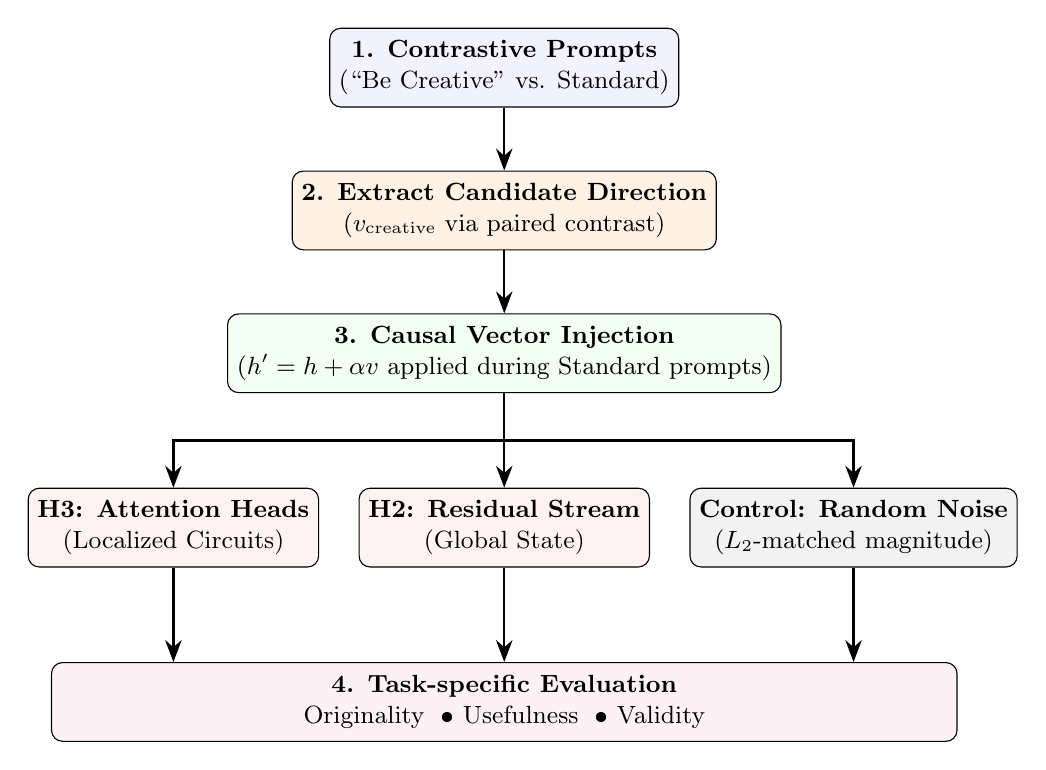
\begin{tikzpicture}[
        node distance=0.8cm and 0.5cm,
        box/.style={rectangle, draw, rounded corners, align=center, minimum width=4cm, minimum height=1cm, fill=blue!5, font=\small},
        trackbox/.style={rectangle, draw, rounded corners, align=center, minimum width=3.5cm, minimum height=1cm, fill=red!5, font=\small},
        arrow/.style={-{Stealth[scale=1.2]}, thick}
    ]

    \node[box] (step1) {\textbf{1. Contrastive Prompts}\\(``Be Creative'' vs. Standard)};
    
    \node[box, below=of step1, fill=orange!10] (step2) {\textbf{2. Extract Candidate Direction}\\($v_{\text{creative}}$ via paired contrast)};

    \node[box, below=of step2, fill=green!5, minimum width=6cm] (step3) {\textbf{3. Causal Vector Injection}\\($h' = h + \alpha v$ applied during Standard prompts)};

    \node[trackbox, below=1.2cm of step3] (h2) {\textbf{H2: Residual Stream}\\(Global State)};
    \node[trackbox, left=0.5cm of h2] (h3) {\textbf{H3: Attention Heads}\\(Localized Circuits)};
    \node[trackbox, right=0.5cm of h2, fill=gray!10] (control) {\textbf{Control: Random Noise}\\($L_2$-matched magnitude)};

    \node[box, below=1.2cm of h2, fill=purple!5, minimum width=11.5cm] (eval) {\textbf{4. Task-specific Evaluation}\\Originality \ \textbullet \ Usefulness \ \textbullet \ Validity};

    \draw[arrow] (step1) -- (step2);
    \draw[arrow] (step2) -- (step3);

    \coordinate (fork) at ([yshift=-0.6cm]step3.south);
    \draw[thick] (step3.south) -- (fork);
    \draw[arrow] (fork) -| (h3.north);
    \draw[arrow] (fork) -- (h2.north);
    \draw[arrow] (fork) -| (control.north);

    \draw[arrow] (h3.south) -- (h3.south |- eval.north);
    \draw[arrow] (h2.south) -- (eval.north);
    \draw[arrow] (control.south) -- (control.south |- eval.north);

    \end{tikzpicture}
    \caption{Overview of candidate-direction discovery and addition experiments. Complementary suppression, bidirectional prompt-boundary patching, held-out task transfer, and capability controls are described in the analysis plan.}
    \label{fig:experimental_design}
\end{figure}

\section{Expected Results and Implications}
\countem
Transferable addition and suppression effects would support a shared causal contributor to creativity-related behavior in the tasks studied. Locating the computations that produce and use this representation would strengthen a mechanistic explanation. Such evidence would not alone establish a universal creativity factor, a complete algorithm for creativity, or a correspondence with human creative cognition.

Failure of a single-direction intervention would constrain that intervention hypothesis, not demonstrate that creativity is noise, nonlinear, or decentralized. Alternative explanations include inadequate measurements, extraction data, token positions, intervention strengths, or statistical precision. A low-dimensional subspace, task-specific mechanisms, or a multi-stage process may warrant subsequent tests.

The intended contribution is an experimentally bounded explanation of a shared process supporting creative performance. A successful low-dimensional intervention may modulate a complex computation rather than replace it. Conclusions about generality will explicitly state the tasks, models, instruction distributions, and quality constraints over which the causal effects replicate.


\endcountem
\textbf{Word count = \thewordcount{}}

\printbibliography



\section{Work Plan}
\countem
\begin{itemize}
    \item \textbf{Week 1-2 (13/07-26/07)}: Finish literature review, make contract.
    \item \textbf{Week 3-4 (27/07-09/08)}: Set up environments for running the models and experiments. Hand in abstract for B\&C review.
    \item \textbf{Week 5-7 (10/08-30/08)}: Implement peer feedback on proposal, gather and clean data for initial experiments. Hand in proposal.
    \item \textbf{Week 8-10 (31/08-20/09)}: Away on holiday.
    \item \textbf{Week 11-12 (21/09-04/10)}: Start running contrastive activation patching to extract the global creative steering vectors from the residual stream. Start writing on introduction and methods sections of thesis.
    \item \textbf{Week 13-14 (05/10-18/10)}: Run causal injection experiments for residual stream and evaluate outputs using semantic distance metrics. Start on results section of thesis.
    \item \textbf{Week 15-16 (19/10-01/11)}: Finish introduction section. Begin exploratory RSA on individual attention heads to identify localized function vectors.
    \item \textbf{Week 17-18 (01/11-15/11)}: If expected results are found on the relation, compare direct prompting results to results obtained with injected activation vector. If unexpected results, further investigation into why these unexpected results are found.
    \item \textbf{Week 19-20 (16/11-04/29)}: Continue on interpretation of results and implications. Finish methods section.
    \item \textbf{Week 21-22 (30/11-13/12)}: Start on discussion section, finish results. Room for some delays on the analysis part.
    \item \textbf{Week 23-24 (14/12-27/12)}: Make first draft of entire thesis, clean up code and finalize experiments.
    \item \textbf{Week 25-26 (28/12-10/01)}: Room for delays, hand in final version of thesis. Plan presentation.
\end{itemize}
\endcountem
\textbf{Word count = \thewordcount{}}

\section*{Signatures}

\vspace{1.5em}

\noindent $\square$ I hereby declare that both this proposal, and its resulting thesis, will only contain original material and is free of plagiarism (cf.\ Teaching and Examination Regulation in the research master's course catalogue).

\vspace{4em}

\noindent
\begin{minipage}[t]{0.3\textwidth}
    \textbf{Location:}\\[3em]
    \makebox[\linewidth]{Amsterdam}
\end{minipage}%
\hfill
\begin{minipage}[t]{0.32\textwidth}
    \textbf{Student's digital signature:}\\[3em]
    \makebox[\linewidth]{\dotfill}
\end{minipage}%
\hfill
\begin{minipage}[t]{0.32\textwidth}
    \textbf{Supervisor's digital signature:}\\[3em]
    \makebox[\linewidth]{\dotfill}
\end{minipage}

\end{document}


\end{document}
